%%%%%%%%%%%%%%%%%%%% chapter1.tex %%%%%%%%%%%%%%%%%%%%%%%%%%%%%%%%%
%
% sample chapter
%
% Use this file as a template for your own input.
%
\chapter{Python Basics}
\label{basics} % Always give a unique label
% use \chaptermark{}
% to alter or adjust the chapter heading in the running head
\section{General Overview}
\label{sec:overview}
This chapter will assume that you have installed a working version of Python 2.7 on your computer. In order to use Python, you have to type commands, and to do so you have several options. First, your installation of Python likely comes with a Python interpreter (on the Enthought Python installation, it is called IDLE). Double-clicking on this application will start a python shell window. Second, you can open (in Linux or OS X) a terminal window and type
\begin{verbatim}
	python
\end{verbatim}
You will then see something like this:
\small\begin{verbatim}
Enthought Python Distribution -- www.enthought.com
Version: 7.1-2 (64-bit)

Python 2.7.2 |EPD 7.1-2 (64-bit)| (default, Jul 27 2011, 14:50:45) 
[GCC 4.0.1 (Apple Inc. build 5493)] on darwin
Type "packages", "demo" or "enthought" for more information.
>>> 
\end{verbatim}\normalsize
The notation \verb">>>" indicates that Python is ready to accept commands, and is an interactive mode.
These first two options are almost identical in their function, so I'll leave it to the reader to choose which is most convenient.
The third option is to use a text editor to write Python code and then compile the code either with the terminal, or, if the text editor is powerful enough, from within the text editor itself. On OS X, there is an excellent editor called TextMate, which excels at this. In fact, TextMate was also the editor used to write the \LaTeX\ code for this book. A cross platform and open source option is Geany. The last option is to use an integrated development environment; there are many programs in this category, but I opt not to use this route because of the overhead needed, and my bias that a closer contact to the code and compilation is better for understanding what is happening when learning to program.

This textbook will use the interactive mode (through either the terminal or IDLE) and compiling text files containing Python code. For short programs, or for developing code, it is convenient to use the interactive mode, as you can get immediate feedback. More on this soon. For the bulk of our work in this text, we will assume you are using a text editor, and write files which are then run by the Python interpreter. Whenever you see the notation \verb">>>", this is an indication that Python is being used interactively, and it's a good idea to try out the examples. 

This chapter will explore the interactive mode, extending Python with external libraries, how to write and compile Python code, and generally provide you with a baseline of tools needed to get started programming so that we can get to the physics as quickly as possible. 

\section{Python as an Interactive Calculator}
\label{sec:calculator}
% Always give a unique label
% and use \ref{<label>} for cross-references
% and \cite{<label>} for bibliographic references
% use \sectionmark{}
% to alter or adjust the section heading in the running head
One of the wonderful features of Python is the ability to use it in an interactive fashion, and also, the simplicity of its syntax. For example, suppose you want to perform a simple calculation such as adding two numbers. Open up a terminal window type \texttt{python} and type \texttt{print 2+5}; you will see the following:
\small\begin{verbatim}
	>>> 2+5
	7
	>>> 
\end{verbatim}\normalsize
Python simply prints the result of the operation, and the interpreter shows a new prompt indicating it is ready for further input. Notice that we simply have added two integers without having to declare them as such. Python makes an intelligent decision based on whether we input integers or floating point numbers; it assumes that if you do not enter a decimal point, that the number is an integer, and otherwise (with the exception of complex numbers) the number is a floating point (called a \verb2float2 in Python parlance). Notice that we have to be careful when dividing as the following examples show (comments are mine):
\small\begin{verbatim}
	>>> 2/5	  # dividing two integers gives the lowest integer
	0
	>>> 5/2	  # same thing here.		
	2
	>>> 5./2   # here we divide a floating point number by an integer
	2.5
	>>> 5/2.   # same here
	2.5
\end{verbatim}\normalsize
Notice that we can put a comment within a line of Python input. A \# sign starts a comment; anything after this character is ignored.

In physics, we often have more complicated arithmetic, such as the expression $\pi\times 10^{7} \cdot \sqrt{90.1}$. This is accomplished as follows: 
\small\begin{verbatim}
	>>> from math import *
	>>> pi*10**7*sqrt(90.1)
	298203178.477 049 65
\end{verbatim}\normalsize
In order to use the value of $\pi$, we have to first load the math library; the statement \texttt{from math import *} loads all of the functions from the math library, including trigometric and logarithmic functions. This will be a standard library to include in most of the Python programs in this book. 
Also notice that Python understands the order of operations, and we did not need parenthesis. The calculation we performed here involves both integers and floating point (i.e. numbers with decimal points) numbers. 

Now, if you are being a skeptical student, you will have checked the previous calculation with your calculator, and verified that it appears to agree (actually, your calculator will likely only give you an answer to the 4th decimal place). However, if you perform the calculation in Mathematica 6.0, and C++, you will find that the answers are 
\small\begin{verbatim}
	298,203,178.477 049 591 064 453 125		(Mathematica 6.0)
	298 203 178.477 049 589 157 104 492 	(C++, gnu compiler)	
\end{verbatim}\normalsize
Notice that these disagree with the Python calculation in the 16th significant digit. In this case, I would likely trust the Mathematica result, as it is specifically designed for high precision calculations. However, the point here, is that Python (and C++, Fortran, etc) have inherent numerical limitations (typically about 16 digits of accuracy for double precision floating point numbers). We have to be careful to not perform calculations where this limitation is significant.

\section{Python libraries: Loading and getting help}
\label{sec:mathlibrary}
As we have already seen, the core of the Python language is easily extensible by loading libraries (most of which are freely available) There are libraries for mathematics, graphing functions, 3d visualization, and many others. Here, we look a little more closely at the math library and how to find out about the available functions. 
%
% For tables use
%
\begin{table}
\centering
\caption{A partial list of constants and functions in the Python math library.}
\label{tab:mathlibrary}       % Give a unique label
\begin{tabular}{ll}
\hline\noalign{\smallskip}
Function\hspace*{7mm} & Description  \\
\noalign{\smallskip}\hline\noalign{\smallskip}
sqrt(x) 		&	Returns the square root of x\\
exp(x)		&	Returns $\exp(x)$ \\
log(x)		&	Returns the natural log, i.e. $\ln(x)$\\
log10(x)	&	Returns the log to the base 10 of x \\
degrees(x)	&	converts angle x from radians to degrees\\
radians(x) 	&	converts angle x from degrees to radians\\
pow(x,y)	&	Return $x^y$; you can also use x**y  \\
hypot(x,y)	&	Return the Euclidean distance, $\sqrt{x^2 + y^2}$\\
sin(x)		&	Returns the sine of x\\
cos(x)		&	Return the cosine of x\\
tan(x)		&	Returns the tangent of x\\
asin(x)		&	Return the arc sine of x\\
acos(x)		&	Return the arc cosine of x\\
atan(x)		&	Return the arc tangent of x\\
atan2()		&   Return the arc tangent of y/x.\\
fabs()		&   Return the absolute value, i.e. the modulus, of x\\
floor()		&   Rounds a floating point number down\\
ceil()		&	Rounds a floating point number up\\
\noalign{\smallskip}\hline\noalign{\smallskip}
Constant 	& 	Description  \\
\noalign{\smallskip}\hline\noalign{\smallskip}
e			& 	$e=2.718...$\\
pi			&	$\pi=3.14159...$\\
\noalign{\smallskip}\hline
\end{tabular}
\end{table}
%

Table~\ref{tab:mathlibrary} lists some of the functions available in the Python math library; in addition, one can always get complete information about the functions available in a given library by using the \verb2help()2 command:\small
\begin{verbatim}
	>>> import math
	>>> help(math)
\end{verbatim}
\normalsize

I haven't printed the output of the help command here to save space, but you should get familiar with this command, as it is a useful feature of Python that applies to other libraries too. Also notice that in order to get help on the elements of a library, one has to import the library (in this case \verb2import math2) in a different manner than we used in to actually access the functions within the library. 

\subsection{Two methods of loading libraries}
\label{sec:LoadingLibraries}
When importing libraries into Python, we have two alternatives (math library used as an example):
\begin{enumerate}
	\item \lstinline2from math import *2
	\item \lstinline2import math2
\end{enumerate}
This text will usually use method (1) which loads all of the functions in the math library. The advantage of this method is that it allows us to call a function by its name in the particular library, for example, to calculate the sine of x, we simply type 
\begin{verbatim}
	sin(x)
\end{verbatim} 

Method (2) also loads the entire math library, but now to calculate the sine of x, we must type
\begin{verbatim}
	math.sin(x)
\end{verbatim}
This method, although it involves more typing, has the advantage of explicitly addressing the function sin() contained in the math library. For instance, you could also have your own function defined (more on functions soon) which was also called sin() and there would be no conflict between the two. Of course, it would be bad programming practice to define your own function with the same name as a known function in the math library, but if it was important to do so, this alternate method of loading the library would allow it. 


However, in order to be able so get help on the contents of the library, we must import the library itself. This is outlined in section~\ref{sec:mathlibrary}. \\
(a) Start a python session using a terminal window or using IDLE. Import the math library and type \verb2help(math)2 as outlined in section~\ref{sec:mathlibrary}. (Do not type \lstinline2from math import *2) If you are using a terminal window (as opposed to IDLE) you need to know the following: the space bar goes to the next page, and the \verb2q2 key exits. Read about the hypot(x,y) command. \\
(b) Now, to evaluate \verb2hypot(3,4)2, you will have to type \verb2math.hypot(3,4)2. Try it and verify that you get the correct answer.\\
So, what's the point of this method of importing the math library? It insures that when you want to use a function specific to that library, you have to expressly indicate so; if we type \lstinline2>>>from math import *2, we have the advantage of being able to address the functions without the \verb2math.func()2 notation, but we run the risk (in a sufficiently complicated program) of defining our own function with the same name. Then, we could get unexpected results. A sufficiently cautious programmer would, I suppose, opt to use the safer \lstinline2import math2 style. Another reason that it is sometimes preferable to use this method, is that it explicitly indicates which library the function is from, which aids in understanding the program or finding documentation (if you import with the * notation, you lose the ability to know which library the function belongs to). This book will mix the two methods, but you are free to use either method in your code.


Problem~\ref{prob1.2} will give you some more experience with using help(math)
as well as exploring some of the functions in the math library.
For a partial list of functions in the math library, see Table~\ref{tab:mathlibrary}. 


\subsubsection{Other Libraries}
\label{sec:OtherLibraries}

There are several Python libraries that we will use in this text; however,  since my goal is to get us thinking about physics as soon as possible, I will discuss their usage as we go. For complete documentation on the Python language, see the  \href{http://docs.python.org/}{Python Library Reference}. Click on the \href{http://docs.python.org/lib/module-sys.html}{Library Reference} link to see full documentation on each library. 

\subsubsection{Alternate Help via pydoc}
\label{sec:pydoc}
Another way to get help---not within a Python session, but on the command line (i.e. a terminal window)---is with \verb!pydoc!, which is included with Python. Typing \verb!pydoc Z!, where \verb!Z! is any function or module within Python's path, will reveal documentation on that item. For example, opening a terminal window and typing \verb!pydoc math.sin!
will reveal documentation on the sine function. 



\section{First Python Program}
\label{sec:FirstProgram}

Let's get started by writing our first Python program that, while not terribly useful, illustrates how to read input and write output to and from the screen. Typically, this is called a ``hello world'' program, but we'll make it a little more interesting by having if actually do something a little more complicated. 

Our first program will simply calculate the vertical position of a ball thrown vertically upward from the surface of Earth at a time $t$ after launch. For simplicity, we make the standard assumptions of constant acceleration due to gravity and no air resistance.
The physics of this motion is simple. The ball's vertical position is given by 
	\begin{equation}
		y(t) = v_0 t - \frac{1}{2}gt^2 .
	\end{equation}
Each program should be proceeded by an outline (or in more complicated programs, a full--blown flowchart illustrating all of the logical steps) that lays out the steps needed. Here is a simple outline for our program:
\begin{enumerate}
	\item Read input velocity, $v_0$ and the time $t$
	\item Compute the position at time $t$
	\item Print out the result
\end{enumerate}
 Here is the Python code needed: \\
\lstinputlisting[
caption={Our First Python Program},
label=FirstProgram, 
style = myPythonStyle]
{Code/4BasicPython/program1.py}

To create a python program with this code, it is helpful to use a Python aware text editor, so that the editor will perform syntax highlighting and formatting specific to Python. On the Mac, I recommend TextMate (shareware) or Smultron, Vi, or Emacs (open source). Another option (which is also cross platform and open source) Having chosen a suitable editor, create a new file and give it a .py extension, or download the file program1.py from the \href{http://www.usm.maine.edu/~pauln/CompPhysPython}{text website}. Decide where you are going to keep your programs, and start off by thinking about a logical scheme. I suggest you create a folder called MyPrograms and place it in your home user folder. Then, since you will likely have many programs in here, it makes sense to have each program in its own subfolder, so that any files or images generated stay organized and associated with the original Python program.

To run the program, open a terminal window (on the Mac, this is in the Applications/Utilities/ folder). Then, before running the program, you have to change your directory (unix command=cd) to your current program folder. To do this, you have two options on the Macintosh: 
\begin{enumerate}
	\item With the terminal window open, type \verb2cd MyPrograms/Program1/2
	followed by the RETURN key. 
	\item With the terminal open, type \verb2cd 2 (with a space after cd) and then drag the folder Program1 (or whatever you have called it) to the terminal window. The Mac OS will copy the address of the folder to the terminal. Then click on the terminal window and press RETURN.
\end{enumerate}
To run the program with an initial upward velocity of 19.6 m/s and a time 3.0 seconds, type
\begin{verbatim}
	python program1.py 19.6 3.0
\end{verbatim}
followed by RETURN.
Python returns the answer of 14.7 meters, as seen in Figure~\ref{fig:FirstPythonProgram}.
\begin{figure}
\centering
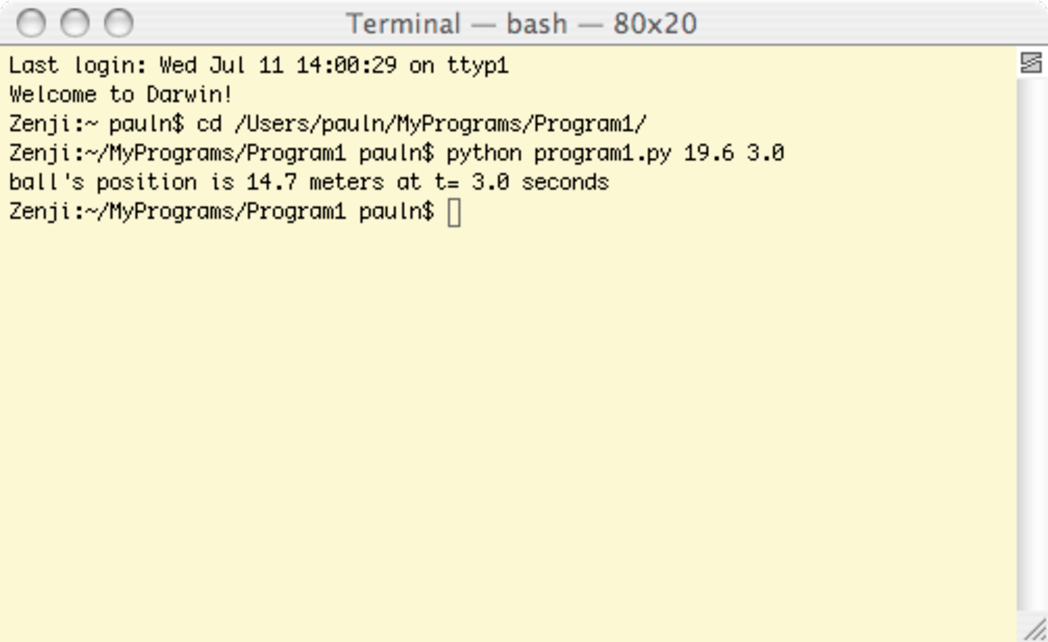
\includegraphics[height=7cm]{Figures/4BasicPython/TerminalWindow1}
\caption{Running our first Python program}
\label{fig:FirstPythonProgram}       % Give a unique label
\end{figure}

\subsection{Discussion of Code}
\label{sec:Program1Discussion}
The first line imports the \lstinline2sys2 (system) library, and which we use in this program to be able to pass input values for the initial velocity and the time to the program. The second line imports all the functions of the math library (which, in this case we don't need, but I include anyway since most programs will need the math library). 

The next section is a \lstinline2try...except:2 block specific to Python which is the standard method for dealing with potential errors. The system library contains a text array called \lstinline2argv[]2; sys.argv[0] contains the name of the python program (sometimes called a script instead), sys.argv[1] and sys.argv[2] refer to other parameters passed to the program (in our case, v0 and t). When Python encounters a \lstinline2try...except2 block, it attempts to execute the elements in the \lstinline2try:2 block, and, if successful, passes control to what follows the \lstinline2except:2 block. 

So, in our case, the program reads the three parameters that you entered when running the program in the terminal: sys.argv[0] is the name of the program (in this case program1.py), sys.argv[1] is defined to be v0, and sys.argv[2] is defined to be t. If an error occurs---for instance, you forget to enter any values for v0 and t when you call the program---then the \lstinline2except:2 block is executed. 

In the case of an error the \lstinline2except:2 block prints out a reminder to the user to call the program with two arguments (v0 and t), and then calls another system routine which exits the program. 

The last portion of the program is only executed when there are no errors, and that consists of a straightforward calculation of the height of the projectile and a simple print statement. In Python, it is acceptable to use either single or double quotes; this example uses double quotes.

Although this first program is very simple, the \lstinline!try:...except:! block is a significant chunk of the script, and the program could be made considerably shorter without it; the script would then be written simply as
\begin{lstlisting}[frame=none, style = pythonSnippet]
	import sys
	from math import *

	v0 = 19.6 		# initial velocity
	t = 3.0			# time			
	y = v0*t-4.9*t**2	#  position 
	print "ball's position is", y, "meters at t=", t, "seconds"
\end{lstlisting}
In this case, the code is clearly more readable, but now, to run the script with different values for the initial velocity and time, the code would have to be edited and saved, and then you would have to execute the script from the terminal once again. Reading the input parameters from the command line using  the  \lstinline!try:...except:! block gives one the ability to re-run the code without going through this extra step. 

Two other comments about Python that we will encounter as we move forward: in Python, we do not have to end lines with semicolons (as in C and C++), and do not have to use braces to demarcate the extent of structured environments. For instance, in this example, the extent of the \lstinline2try2 and of the \lstinline2except:2 blocks are completely demarcated by the indentation. So, it is critical to be very careful with indentation in Python. It makes for very easy to read code, but forces the programmer to be mindful of indentation when coding. The second comment is that you should get in the habit of using comments to explain your code and make it readable to other users (and yourself). Comments in Python are preceded by a \# sign; anything on the line after this character is ignored. Commenting your code achieves several things; it makes you explain your code (which often catches errors in reasoning), and it makes your code easier to decipher, especially when others may not understand your choice of variables. 

\section{Second Python Program}
\label{sec:SecondProgram}

Now that we have written a simple Python program, we are ready to add more to our toolbag. Lets see how to incorporate graphics into our output; we'll modify our program to plot the vertical position of the ball as a function of time. In doing so, we will also learn about loop structures, reading and writing data to files, and the MatplotLib plotting library. Here is the Python script that accomplishes this. 

\lstinputlisting[caption={Our second Python program adds graphical output using MatPlotLib.}, label={SecondProgram}]{Code/4BasicPython/program2.py}

\subsection{Running the script}
\label{subsec:running}

Once you've created a file with the above code, save the file as \verb!program2.py! and then open a terminal window. Change your directory to the folder containing your script; let's assume you place the script in a folder \verb!Program2! which is a subfolder of the \verb2MyPrograms2 folder in your home directory. Then type
\begin{verbatim}
	cd MyPrograms/Program2/
\end{verbatim}
and then, assuming that you want to create a data file called \verb2trajectory.dat2, and you want to launch the ball upward at 19.6 m/s, plot the vertical position for 4 seconds, and plot points every 0.1 seconds, you would type 
\begin{verbatim}
	python program2.py 'trajectory.dat' 19.6 4.0 0.1
\end{verbatim}
Python will create the data file, and display the graphic shown in 
Figure~\ref{fig:SecondPythonProgram}. 
\begin{figure}
\centering
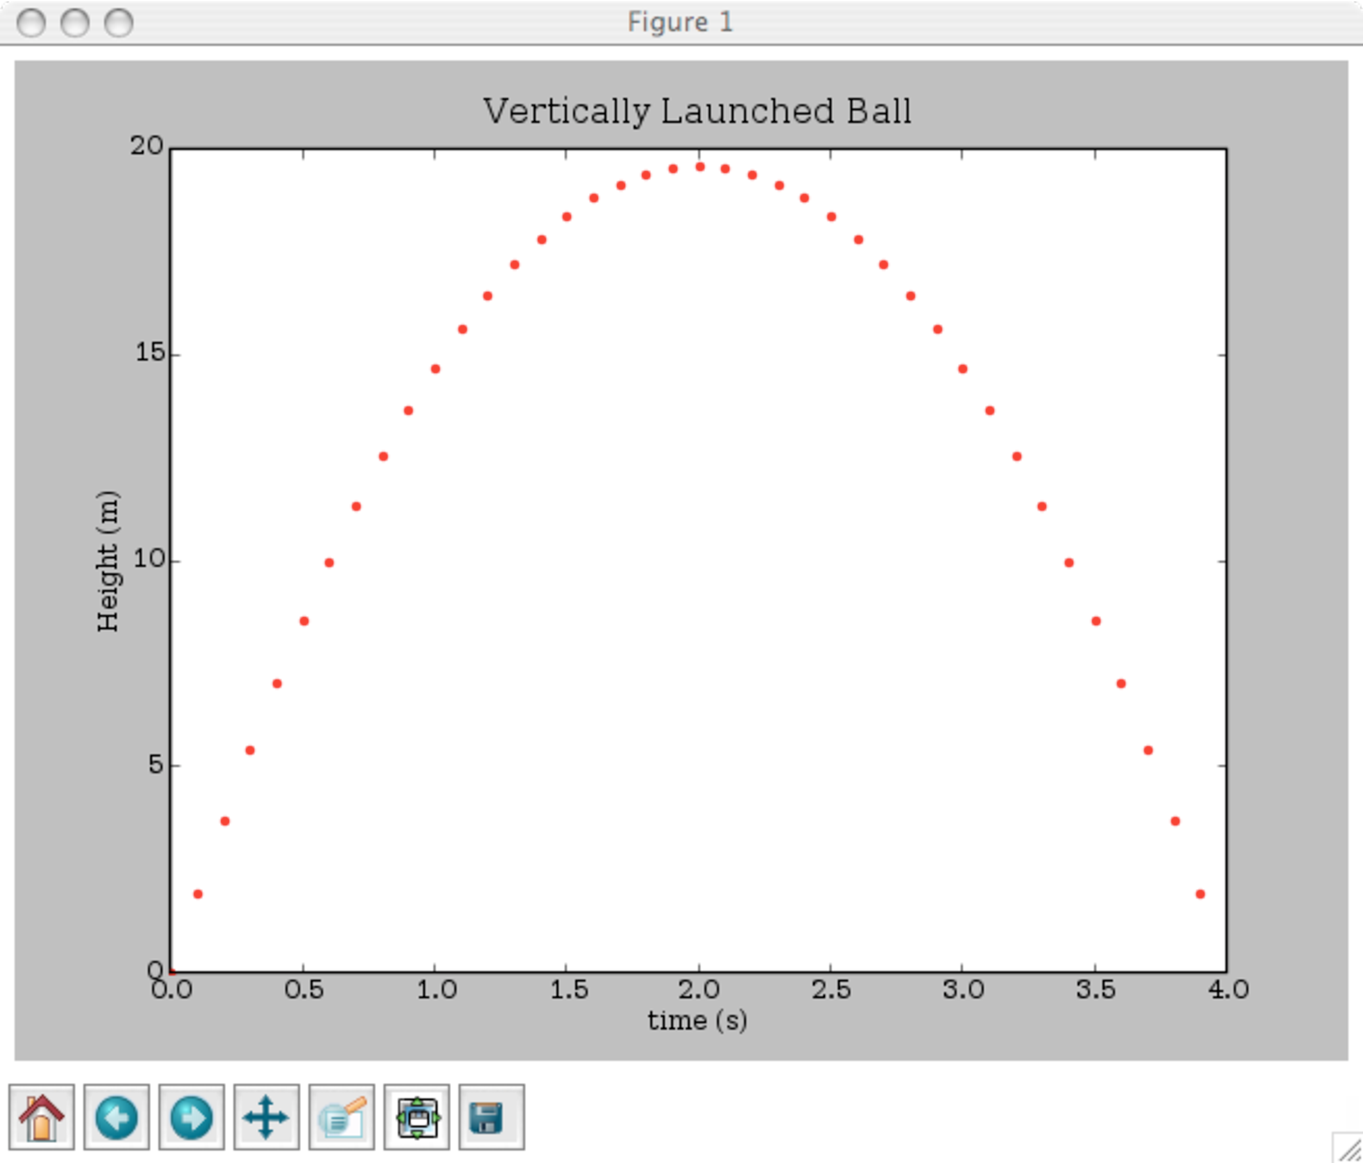
\includegraphics[height=8cm]{Figures/4BasicPython/trajectory.pdf}
\caption{MatplotLib output from our second Python script. Clicking the bottom rightmost disk icon at the bottom of the plot will save the figure as a .png file. To return control to the terminal, simply close the window. Explore the other buttons to see some of the interactive features provided with every Matplotlib figure.}
\label{fig:SecondPythonProgram}       % Give a unique label
\end{figure}

\subsection{Discussion of the Script}
\label{subsec:DiscussionOfScript}

Our second Python script starts by an extended comment (the triple quotes demarcate a special comment called a docstring, which is useful in documenting this piece of Python code. More on this in a later chapter. Then the script procedes by loading the libraries we will need. The system (sys) library for reading and writing data, and the pylab library for accessing Matplotlib, which is a Matlab-like plotting library. The distinction between pylab and Matplotlib is actually a bit unclear to this author, as even the Matplotlib web site presents the two packages as synonymous, however, it will not work in this case to replace \verb!from pylab import *! with \verb!from matplotlib import *!. 

The next block of code uses a  \lstinline!try:...except:! block to read in the output file name, the initial velocity, the length of time to follow the ball, and the time step. 

After reading in these parameters from the terminal, we define \verb2outfile2 to open an output file to write data to:
\begin{verbatim}
	outfile = open(outfilename, 'w')
\end{verbatim}
where \verb2open2 is a system library function that opens creates the file, and \verb2outfile2 is an arbitrary user create variable. If there is a need to write multiple output files, then one must create a variable to point to each file. The \verb2'w'2 indicates that the file is prepared for being written to; if we wanted to open a file for reading, we would use \verb2'r'2 instead of \verb2'w'2. We then define the acceleration due to gravity, and set the start time to 0 seconds. 

Now, we introduce a new structure called a function. We define a function called \verb2height(v0,t)2 which has two inputs, the initial velocity, and the time. Within this function, we have a decision structure called an \verb2if...else2 statement. In our example, if the initial velocity is greater than zero, then the function \verb2height(v0,t)  returns2 the height of the ball at time t using the standard kinematic result. If the ball's initial velocity is less than or equal to zero, then a statement to this effect is printed to the terminal, and the program exits. 

Notice that the extent of the body of the function is demarcated by the indentation; the blank line after \verb2sys.exit(1)2 is purely for a visual readability of the code. In addition, indentation also governs the extent of the \verb2if...else2 statement. Note that Python executes code sequentially, so that the function \verb2height()2 must be defined \textit{before} it is used; for example, it won't do to place this function at the end of the script---Python will give an error if this occurs. 

The next line writes the column labels, \verb2time (s)2 and \verb2height (m)2, as the first line of \verb2outfile2. Between these column headings is a tab character, represented as \verb2\t2, and at the end is a newline character, \verb2\n2. 

The physics in this program is in the main calculation loop. First I calculate the number of steps needed to iterate over given a time of \verb!tmax! and a time step of \verb!dt!.

The main calculation is a loop that uses a \verb2for2 statement. This statement tests a condition, and if true, executes the body of the loop (demarcated by indentation, of course). In our case, we use Python's \verb2range()2 function, which has three possible forms:
\begin{enumerate}
	\item range(n) : returns a list of integers from 0 to n-1 
	\item range(a,b): returns a list of integers from a to b-1
	\item range(a,b,dn): returns a list of integers from a to (b-dn) in incements of dn.
\end{enumerate}
For example: 
\begin{verbatim}
	>>> range(3)
	[0, 1, 2]
	>>> range(1,3)
	[1, 2]
	>>> range(1,10,2)
	[1, 3, 5, 7, 9]
\end{verbatim}
So, the \verb2for2 statement starts with i=0, evaluates the next three lines, then reads the next value of i, executes the three lines again, reads the next value of i, etc. 
Execution of the loop ceases after evaluating the loop for the i=imax-1, then the output file is closed. So, in our code, in order to plot points from \verb!t=0! to \verb!t=tmax!, we must have our for statement read
\begin{lstlisting}[frame=none]
	for i in range(imax+1)
\end{lstlisting}
otherwise, we will end up one time step short of the maximum. This (at least to me) is a slight annoyance of Python (an C/C++ too), but we are stuck with this fact that indexing starts from zero in Python. The rest of the \verb!for! loop calculates the time, the height (using our defined function \verb!height()!), and then writes out the time and height to our output data file, one line at a time. Notice that the write statement
\begin{lstlisting}[frame=none]
	outfile.write('%g \t %g\n' % (t,y))
\end{lstlisting}
consists of two pieces. The first 
\begin{verbatim}
	'%g \t %g\n'
\end{verbatim}
is called a format string, and it defines that two numbers are to be written to the output file. The first number is a floating point (\verb!%g!), followed by a tab character (\verb!\t!), another floating point number, and finally, a newline character (\verb!\n!). This format string is inherited from the C programming language; at its most basic level, a format string has the form
\begin{verbatim}
	%<width>.<precision><type-character>
\end{verbatim}
where the width and precision are optional arguments, and not all formats (shown in Table~\ref{tab:FormatSpecifiers}) can accept width and precision arguments. For example, if x=1234.5678 the format string 
\begin{verbatim}
	%10.4f
\end{verbatim}
indicates that a floating point number with 10 digits will be written with 4 decimal places shown. Since x has 9 characters (the decimal point counts as one character), the above print statement will pad the output with one blank space at the left. On the other hand, the \verb!%g! format is a \textit{general} format specifier that defaults to a precision (read:\# significant figures) of 6. To specify the number of significant figures with the \verb!%g! format, the width argument is irrelevant, and the precision argument specifies the number of significant figures. So, if x=1234.5678, a Python terminal session will produce the following:
\begin{verbatim}
	>>>print '%10.4f \n' % x 
	 1234.5678				# note the space at the left
	>>>print '%9.4f \n' % x 
	1234.5678
	>>>print '%g \n' % x 		# %g defaults to 6 signif. figs
	1234.567
	>>>print '%.6g \n' % x 		# same as default!
	1234.567
	>>>print '%.7g \n' % x 		
	1234.568
	>>>print '%.8g \n' % x 		# now the full number is shown
	1234.5678
	>>>print '%.8f \n' % x 		# this will show 8 decimal places
	1234.56780000				
\end{verbatim}

If you ever want to see the result of a particular formatting statement, you can always see the results in an interactive terminal session---one of the benefits of Python over compiled languages. For reference,  Table~\ref{tab:FormatSpecifiers} shows a list of common format specifiers.
\begin{table}
\centering
\caption{A partial list of format specifiers in Python. For more information, see the \href{http://docs.python.org/}{Python Documentation}, click on Library
Reference, and search for \href{http://docs.python.org/lib/typesseq-strings.html}{String Formatting Operations}. }
\label{tab:FormatSpecifiers}       % Give a unique label
\begin{tabular}{ll}
\hline\noalign{\smallskip}
Specifier\hspace*{7mm} & Description  \\
\noalign{\smallskip}\hline\noalign{\smallskip}
d&	Signed integer decimal.	\\
i&	Signed integer decimal.	\\
o&	Unsigned octal.\\
u&	Unsigned decimal.\\	
x&	Unsigned hexadecimal (lowercase).\\
X&	Unsigned hexadecimal (uppercase).\\
e&	Floating point exponential format \\
E&  Same as \verb!%e! except an upper case E is used for exponent.\\
f&	Floating point decimal format.\\
g&	Floating point format. Uses exponential format if exponent is\\
 & greater than -4 or less than precision, decimal format otherwise.\\
G&  Same as \verb!%g! except an upper case E is used for the exponent.\\
c&	Single character (accepts integer or single character string).	\\
r&	String (converts any python object using repr()).	\\
s&	String (converts any python object using str()).\\
\noalign{\smallskip}\hline
\end{tabular}
\end{table}
%

The last portion of the program uses pylab/matplotlib to read the data and plot it to a new window on the computer The \verb!load! command is from the pylab library; remember, you can get help on this command by opening a terminal window, and typing 
\begin{verbatim}
$ python
>>> import python
>>> help(pylab.load) .
\end{verbatim}
The lines
\begin{lstlisting}[frame=none]
xaxis = data[ : , 0 ]			# first column
yaxis = data[ : , 1 ]			# second column
\end{lstlisting}
define two lists \verb!xaxis! and \verb!yaxis! to be the first and second columns of the array \verb!data!. Note that because python starts arrays with index zero, the first column is column 0. The remaining commands use \verb!Matplotlib! to plot these two lists. Notice that the plot produced comes with a toolbar along the bottom of the display. Your should experiment with them to see what options they present (one of them is to save a copy of the plot to disk). To exit the plot and return control to the terminal, you have to close the window. 

There are many more features of Matplotlib; if you are eager to see more, you can see the \verb!Matplotlib! \href{http://matplotlib.sourceforge.net/tutorial.html}{tutorial}, and for a complete reference, see the \href{http://matplotlib.sourceforge.net/}{User's Guide} at the \verb!Matplotlib! home page. We will learn to use other features of this plotting library as we progress forward. 

\section{Saving Functions as Modules}
\label{sec:Modules}
Although our second program (~\ref{SecondProgram}) is not terribly complicated, as we develop more involved codes, it is good practice to modularize our code. There are two primary ways to accomplish this; one is to use the object--oriented features of Python and another is to split off functions into separate pieces of Python code called \href{http://docs.python.org/tut/node8.html}{modules}. For example, we can split the function \verb!height(vo,t)! from our main script, and save it as a separate file; however, it is a good idea to make a small change to the \verb!height! routine by adding an option for the acceleration due to gravity, with g=9.8 m/s$^2$ being a default value. Here is the modified \verb!height()! routine, saved as \verb!analytic.py! (named both to remind us that this is the analytic solution for the height, and to avoid an awkward function call):
%
\lstinputlisting[caption={Sections of code can be saved as reusable functions}, label=snippet]{Code/4BasicPython/analytic.py}
% 
If we wanted to call the height function from our main program, we have to make sure to place \verb!analytic.py! in the same folder as \verb!program2.py!, and make sure to import it either by \\
\verb!import analytic!\\
or \\
\verb!from analytic import height! (or \verb!from analytic import *!).\\
Then, to call the function, we have to use either analytic.height(v0,t), or height(v0,t), respectively. Notice that due to the inclusion of g=9.8 in the definition of the function, we do not need to pass the acceleration due to gravity; however, if we wanted to, we could alter the value of g in the function call by, for instance, \verb!height(v0,t,g=4.9)!. 
Here is the code of Listing~\ref{SecondProgram} modified to use our function \verb!height()! which is included in the file \verb!analytic.py!:
%
\lstinputlisting[caption={Our first program made modular.}, label=ThirdProgram]{Code/4BasicPython/program2_mod.py}
%


\section{Other Data Types in Python}
\label{sec-datatypes}
Although we will primarily be using floating point numbers and integers, Python also has several other data types that we will use: Boolean, complex numbers, strings, and lists. 
\subsection{Boolean Integers}
\label{subsec-boolean}
A boolean variable in Python is actually an integer; either False (0) or True (1), which you can see if you attempt to use them as in a numerical context. The following examples illustrate the use of booleans: 
\begin{verbatim}
	>>> b=1<2 
	>>> b
	True
	>>> b+1
	2
	>>> bool(b)
	True
	>>> bool(20<100)
	True
	>>> bool(20<=19)
	False
	>>> bool(20<=20)
	True
\end{verbatim}
\subsection{Complex Numbers	}
\label{subsec-complex}
Complex numbers in Python are created by one of two methods: 
\begin{lstlisting}[frame=none]
a=1.0 + 2.0j 	# you can also use uppercase J if you like
a=complex(1,2)
\end{lstlisting}
and the real and imaginary parts are represented internally as floating point numbers (even if you type them without a decimal point). You can extract the real and imaginary parts and obtain the modulus  as follows:
\begin{lstlisting}[frame=none]
>>> z=3 + 4j 
>>> z.real
3.0
>>> z.imag
4.0
>>> abs(z)
5.0
\end{lstlisting}

\subsection{Strings}
\label{subsec-strings}
Strings are simply sequences of alphanumeric characters, and in Python, can be enclosed in single or double quotes. You can also refer to a specific character by its position in the sequence, and can also easily extract a range of characters:
\begin{lstlisting}[frame=none]
>>> x='Ministry of Silly Walks'
>>> x
'Ministry of Silly Walks'
>>> x[0]
'M'
>>> x[5]
't'
>>> x[0:8]
'Ministry'
\end{lstlisting}
You can also add a character to a string in a straightforward manner:
\begin{lstlisting}[frame=none]
>>> y=x+'!!'	# creates a new string with added exclamation points
>>> y
'Ministry of Silly Walks!!'
>>> z=y[ :-2]	# creates a new string which is every character from
>>> z		# y except the last two characters.
'Ministry of Silly Walks'
\end{lstlisting}
Being able to add a character(s) to a string is especially convenient when writing a series of output files with slightly different names. 

\subsection{Lists}
\label{subsec-lists}
A list is a compound data type composed of several comma-separated values enclosed by square braces; the individual elements need not be of the same data type:
\begin{lstlisting}[frame=none]
>>> misc=['silly', 8, 2.0, 3.0 + 4.0j]
>>> misc[0]		# extracts first element of misc
'silly'
>>> misc[1]*misc[2]	# you can multiply elements together if appropriate
16.0
>>> misc[1]*misc[3]	# even this is okay
(24+32j)
>>> misc[-1]	# displays last element
(3+4j)
>>> new=misc + ['walk', 3.14]	# create new list 
>>> new
['silly', 8, 2.0, (3+4j), 'walk', 3.1400000000000001]
>>> len(new)	# the number of elements in the list
4
\end{lstlisting}
There are many other features of lists, and we will introduce them as needed.


\section{Flow Control: if, while, for}
\label{sec-flow}
There are three main ways to control the flow of program execution in Python. We will look briefly at each. 

\subsection{if Statements}
\label{subsec-if}
The if-statement has the general form 
\begin{lstlisting}[frame=none]
	if <expression is true> :
		then execute
		each indented line
	otherwise continue on to next unindented line
\end{lstlisting}
Here is a simple example:
\begin{lstlisting}[frame=none]
i=10
if i <= 100:	# note colon at end of line
	i=i+1
print i
\end{lstlisting}
Running the above will print out a result of 11 for i. 

Often, a single \verb!if! statement is not sufficient, so Python provides for \verb!if!\ldots \verb!else!
 and \verb!if!\ldots \verb!elif!\ldots \verb!elif! \ldots structures. The \verb!else! portion is optional, and \verb!elif! is short for \verb!else if!. The logic is fairly straightforward, as this simple example shows: 
\begin{lstlisting}[frame=none]
i=100	#note that one equals sign assigns the value 100 to i.
if i < 100:
	print 'i<100'
elif i==100:	#note that two equals signs are needed to test for equality
	print 'i=100'
elif i>100:
	print 'i>100'
else:
	print 'it is not possible to get here!'	
\end{lstlisting}

\subsection{while Statements}
\label{subsec-while}
\verb!while! statements are used to iterate over a range of values. The extent of the loop is controlled by indentation, and the loop executes repeatedly until the condition is no longer true. \verb!while! loops have the general format
\begin{lstlisting}[frame=none]
	while <expression is true> :
		execute each indented line
		return to the beginning
		of the while loop to retest 
		the condition. When the test fails,
	exit the loop to the next un-indented line
\end{lstlisting}
Here is a simple example that sums the integers from 0 to 100:
\begin{lstlisting}[frame=none]
	i,sum =0,0	# we can assign values to i and sum simultaneously
	while i<=100:
		sum=sum+i
		i=i+1		
	print sum
\end{lstlisting}
This code properly prints out the sum as 5050, which is obviously correct, since there are 50 sets of 101 (1+100, 2+99, 3+98, \ldots). 

\subsection{for Statements}
\label{subsec-for}
The \verb!for! statement in Python iterates over all of the items in a sequence (which can be a list of numerical values, or even a list of string variables). Typically, for numerical programming, we will make use of the \verb!range()! function as discussed in Section~\ref{subsec:DiscussionOfScript}. Here is an example that sums the integers from 0 to 100 using a \verb!for! statement:
\begin{lstlisting}[frame=none]
	i,sum =0,0	
	for i in range(101):	# note that range(101) consists
		sum=sum+i	# of integers from 0 to 100
		i=i+1		
	print sum
\end{lstlisting}



\section{General Guidelines for Programming}
\label{sec-programmingGuidelines}
Writing a Python script or program is necessarily an individualistic endeavor; those of you just learning the language will clearly write different programs than those who have previous experience. However, There are several guidelines that are good to follow: 
\begin{itemize}
	\item Start each program with a pen and paper outline of its structure. For simple programs, this can be a short bit of pseudo code (just a brief outline of the logical steps the script needs to accomplish); for more complicated programs, you will need to actually create a flowchart that explicitly outlines the many logical steps needed. 
	\item When it comes to writing code, get in the habit of using a logical format; here is a structure suggested by Wesley J. Chun in his book \textit{Core Python Programming}\cite{chun2007}:
	\begin{enumerate}
		\item Startup line (Unix; \verb2#!/usr/bin/env python2)
		\item module documentation (this is what appears between the triple quotes)
		\item module imports (import statements)
		\item variable declarations 
		\item class declarations (we'll get to this later)
		\item function declarations 
		\item main body of program
	\end{enumerate}
	
	\item Comment your code as you write. Ideally, your comments should be sufficient for someone else (assumed to be proficient in Python) to understand your code. 
	
	\item Strive for clarity in your code. Especially as you are first learning to program, there is a temptation to include fancy programming techniques. \textbf{Don't}. After you are sure your code produces reasonable results (see the next item!), then you can (if it is worth the time and effort) optimize your code for speed and add new features. 
	
	\item Always be skeptical of your program's output and check it by testing it for trivial cases where you know an analytical result. For instance, in our second program, even though we were simply computing a known analytic solution for a vertically launched projectile, notice the values I input were an initial velocity of 19.6 m/s and a run time of 4.0 seconds; a quick calculation reveals that the ball should hit the ground at t=4 seconds, and this is reflected in Figure~\ref{fig:SecondPythonProgram}. Checking your program's validity is one of the most important steps in computational physics and a considerable effort should be made to insure that it is working properly before you move on to apply the code to regions that do not admit of analytical results. 
	
	\item Modularize your code and/or use object oriented programming when possible. Modularization improves your code's clarity as well as providing code that can be used by other programs. As we have seen, separating off functions into modules is very easy in Python. Object oriented programming is also easy to implement in Python, but we leave this to a later chapter. \marginpar{What chapter?}	

\end{itemize}

\section{Python References}
\label{sec-references}
For Python, I recommend that everyone have a copy of Guido van Rossum's book\cite{guido-introduction} \href{http://www.network-theory.co.uk/docs/pytut/}{An Introduction to Python} handy; this book is available for purchase as a standard paperback, a downloadable pdf file, or is available for reading online. Many more details about Python are clearly covered in his introduction. Guido is the author of the Python language, and is its BDFL (Benevolent Dictator for Life). If you need more detail, see his complete documentation for Python at the \href{http://www.python.org/doc/}{Python web site}. Keep in mind that although I have only discussed the very basics of the language, Python is a very rich programming language, and if there is something you wish you could do, it's probably possible. 

Two other introductory books can are by John Zelle\cite{zelle} and an excellent introduction and reference by Wesley Chun\cite{chun2007}. At a more advanced level, but very geared toward computational physics is Hans Petter Langtangen's \textit{Python Scripting for Computational Science}\cite{langtangen-3ed}. At the writing of this book, the book is was in its second edition, with a third edition underway. Highly recommended.


\pagebreak
%
%
% Problems or Exercises should be sorted chapterwise
\section*{Problems and Tutorials}
\addcontentsline{toc}{section}{Problems}
%
% Use the following environment.
% Don't forget to label each problem;
% the label is needed for the solutions' environment
\begin{prob}
\label{prob1.1}

\textbf{Interactive Python}\\
Use Python interactively to evaluate the following mathematical expressions, and compare to what you would calculate exactly by paper and pencil:\\
(a) $7.5 + \frac{5}{2}$ \hfill (b) $2.0*(3.0\times 10^8)^2$\hfill (c) $tan(\frac{\pi}{4})$ \hfill (d) $3\times 10^{-7}\log (1000)$\\
(e) $\sin(90^o)$\hfill (f) $\cos(\frac{\pi}{2})$\hfill (g) $\ln(e)$\\

\end{prob}

\begin{prob}
\label{prob1.2}
\textbf{Using Python Help}\\
When importing libraries into Python, we will generally use the method described in section~\ref{sec:calculator}. The advantage of this method is that it allows us to call a function by its name in the particular library, for example, to calculate the sine of x, we simply type \lstinline2sin(x)2. However, in order to be able so get help on the contents of the library, we must import the library itself. This is outlined in section~\ref{sec:mathlibrary}. \\
(a) Start a python session using a terminal window or using IDLE. Import the math library and type \lstinline2help(math)2 as outlined in section~\ref{sec:mathlibrary}. (Do not type \lstinline2from math import *2) If you are using a terminal window (as opposed to IDLE) you need to know the following: the space bar goes to the next page, and the \lstinline2q2 key exits. Read about the hypot(x,y) command. \\
(b) Now, to evaluate \lstinline2hypot(3,4)2, you will have to type \lstinline2math.hypot(3,4)2. Try it and verify that you get the correct answer.\\
(c) Read about the atan2() function using help. Evaluate the arc tangent of a vector with x and y components of -2 and +3 respectively. Why is this a useful function (compared to atan()?)

\end{prob}

\begin{prob}
\label{prob1.3}
\textbf{Matplotlib}\\
Write a simple Python program to make a plot of $\cos(2\pi t)$ from t=0 to t=$4\pi$. Hint: look at the \href{http://matplotlib.sourceforge.net/}{Matplotlib web page} and see the \href{http://matplotlib.sourceforge.net/screenshots.html}{screenshots} link for examples complete with code.
\end{prob}

\begin{prob}
\label{prob1.4}
\textbf{Practice with loops, writing to a file, and Matplotlib}\\
(a) Write a simple Python program to print out the Fibonacci series up to some specified maximum integer, N. \\
(b) Now alter the program so that the maximum number N is read from the command line and the Fibonacci numbers are printed out to a file and plotted with Matplotlib. 

\end{prob}

%
